Modularization concepts increase the flexibility of plants in the process industry. The plant operator is faced with the challenge of no longer being able to solve problems on the basis of extensive experience\footnote[1]{Romy Müller. \glqq Cognitive challenges of changeability: adjustment tosystem changes and transfer of knowledge in modular chemical plants\grqq. In: \textit{Cognition, Technology and Work} 21.1 (2018).}. Assistance systems can relieve people of many tasks and accompany them through a problem-solving process. The analysis of this thesis shows the complexity of the influencing factors on problem and solution. The user is supported by the interaction platform developed ensure that he still has an overview at all times. The interaction platform draws attention to the relevant information. Among experts, the simple operation of the system and the clarity of the solutions receives a very positive response and would be recommended by them.

\vspace{10pt}
\begin{center}
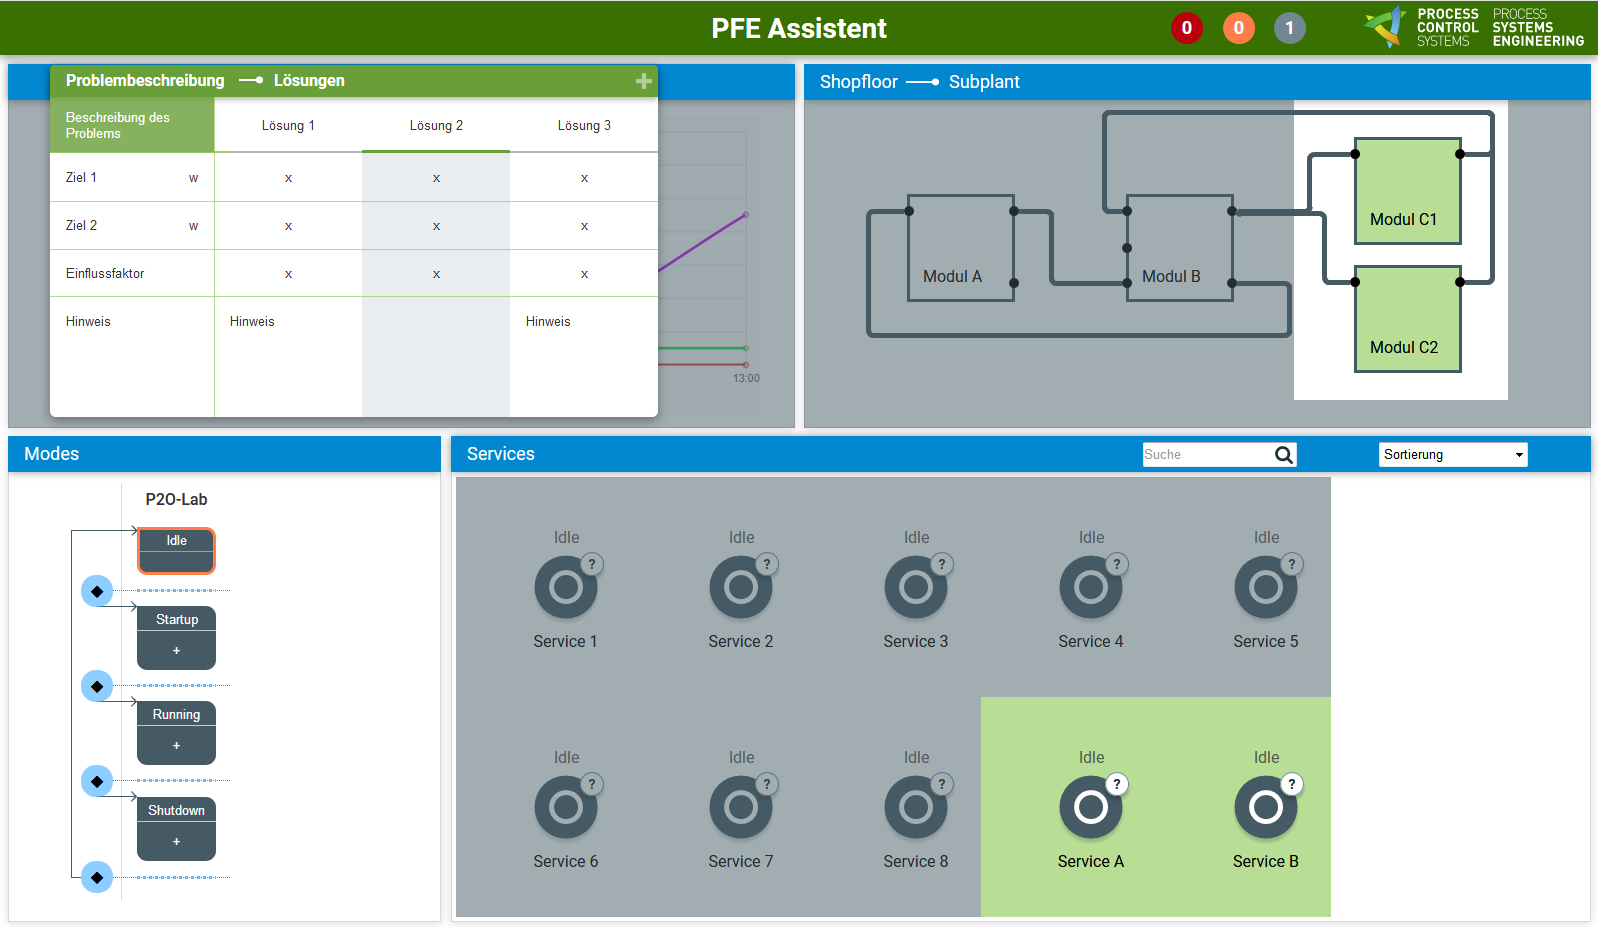
\includegraphics[scale=0.25]{DA_files/Bilder/Konzept/Skizze-Loesungen-PFE.png}
%[keepaspectratio, width=13 cm]
\end{center}
\vspace{6pt}